\documentclass[a4paper, 11pt]{report}
\author{Valentin Clement}
\title{CLAW Fortran Compiler - Developer's Guide}

\usepackage[utf8]{inputenc}
\usepackage{verbatim}
\usepackage{moreverb}
\usepackage[english]{babel}
\usepackage[T1]{fontenc}
\usepackage{lmodern}
\usepackage{graphicx}
\usepackage{fancyhdr}
\usepackage{listings}
\usepackage{lastpage}
\usepackage[top=2cm, bottom=1cm, left=2cm, right=2cm]{geometry}
\usepackage{color}
\usepackage[table]{xcolor}
\usepackage{graphicx}
\usepackage{lipsum}
\usepackage{pgfplots}
\usepackage{CJKutf8}
\usepackage{glossaries}
\usepackage{xspace}

\setcounter{secnumdepth}{3}

\def\fortran{FORTRAN\xspace}
\def\clawfcomp{CLAW FORTRAN Compiler\xspace}
\def\omni{OMNI Compiler Infrastructure\xspace}
\def\xcodeml{XcodeML/F\xspace}
\def\ffront{\lstinline!F_Front!\xspace}
\def\fback{\lstinline!F_Back!\xspace}
\def\fpp{\lstinline!FPP!\xspace}
\def\clawfc{\lstinline!clawfc!\xspace}
\def\cx2x{\lstinline!CX2X!\xspace}

\makeglossaries

\newacronym{ast}{AST}{Abstract Syntax Tree}
\newacronym{ir}{IR}{Intermediate Representation}


%font change
\renewcommand{\familydefault}{\sfdefault}

\newcommand{\HRule}{\rule{\linewidth}{0.5mm}}
\newcommand{\nl}{\\[0.1cm]}
\newcommand{\s}{\vspace{0.3cm}}
%\newcommand{\emptypage}{\newpage \thispagestyle{empty} \mbox{}\newpage}
\newcommand{\emptypage}{}
\newcommand{\smore}{\vspace{0.6cm}}

\usepackage{caption}
\DeclareCaptionFont{white}{\color{white}}
\DeclareCaptionFormat{listing}{\colorbox{gray}{\parbox{\textwidth}{#1#2#3}}}
\captionsetup[lstlisting]{format=listing,labelfont=white,textfont=white}

\definecolor{darkgreen}{rgb}{0,0.4,0}
\definecolor{mauve}{rgb}{0.58,0,0.82}
\definecolor{Gray}{rgb}{0,0,0}
\definecolor{LightGray}{gray}{0.9}


\lstset{
    basicstyle=\footnotesize\ttfamily,
    keywordstyle=\color{orange}, %keywordstyle=\color{MidnightBlue}\bfseries,
    identifierstyle=\color{black},
    commentstyle=\color{darkgreen},
    stringstyle=\color{red},
    numbers=left,
    numberstyle=\color{Gray}\tiny,
    frame=bt, %frame=single,
    rulecolor=\color{Gray},
    numbersep=7pt,
    extendedchars=true,
    captionpos=b,
    breaklines=true,
    showspaces=false,
    showtabs=false,
    tabsize=2,
    xleftmargin=20pt,
    framexleftmargin=20pt,
    framexrightmargin=0pt,
    framextopmargin=0pt,
    framexbottommargin=0pt,
    showstringspaces=false,
    aboveskip=20pt,
    belowskip=20pt
}

\lstset{
	emph={parclass, sync, async, broadcast, scatter, gather, reduce, seq, conc, mutex},
	emphstyle={\color{orange}\bfseries}
}

\addto\captionsenglish{%
  \renewcommand{\listfigurename}{List of figures}%
	\renewcommand\refname{}
}

%Header and footer
\pagestyle{fancy}
\fancyhead{}
\fancyfoot{}

%Header definition
\renewcommand{\headrulewidth}{0.5pt}
\lhead{CLAW FORTRAN Compiler}
\rhead{Developer's Guide}

%Footer definition
\renewcommand{\footrulewidth}{0.5pt}
\lfoot{Version 0.1}
\rfoot{Page \thepage ~on \pageref{LastPage}}

\definecolor{grey}{rgb}{0.9,0.9,0.9} % Color of the box surrounding the title - these values can be changed to give the box a different color	

%remove indent for paragraph
\parindent0ex

\begin{document}

\thispagestyle{empty} % Remove page numbering on this page

%----------------------------------------------------------------------------------------
%	TITLE SECTION
%----------------------------------------------------------------------------------------
\colorbox{grey}{
	\parbox[t]{1.0\linewidth}{
		\centering \fontsize{35pt}{80pt}\selectfont % The first argument for fontsize is the font size of the text and the second is the line spacing - you may need to play with these for your particular title
		\vspace*{2cm} % Space between the start of the title and the top of the grey box
		
		\hfill \textbf{CLAW FORTRAN Compiler} \\
		\hfill Developer's Guide\par
		
		\vspace*{2cm} % Space between the end of the title and the bottom of the grey box
	}
}

\vfill

\begin{center}

\includegraphics[width=4cm]{resources/c2sm_logo.pdf} \\
\end{center}

\vfill % Space between the title box and author information

\begin{center}
Version 0.1, Last updated \today
\end{center}
\HRule

\clearpage % Whitespace to the end of the page



\newgeometry{top=3cm,bottom=3cm,right=2cm,left=2cm}

%\emptypage
%\pagebreak
%\label{chapter:ack}
%\begin{center}
%\textsc{\LARGE Acknowledgment}
%\end{center}
%\input{acknowledgment}

%\emptypage
%\pagebreak
%\label{chapter:abstract}
%\begin{center}
%\textsc{\LARGE Abstract}
%\end{center}


\emptypage
\pagebreak
\tableofcontents



\chapter{Architecture}
\section{OMNI Compiler}
The \clawfcomp is based on the \omni. 

\section{\xcodeml}
\xcodeml is the \gls{ir} used by the translator in the CLAW FORTRAN Compiler. This \gls{ir} is based on the XML format and is described in a specification document. It allows to have an high-level representation of FORTRAN 2008 programs.
%TODO add reference to specs.

Listing \ref{fortran1} is a simple FORTRAN program. Its \xcodeml \gls{ir} will be as shown in Listing \ref{xcodeml1}. A typical \xcodeml translation unit is composed of the followings sections: 
\begin{itemize}
\item Type table with all the type definitions used in the translation unit (Listing \ref{xcodeml1} line 6-24).
\item Global symbol table listing all the symbol at global scope (Listing \ref{xcodeml1} line 25-29).
\item Global declaration section listing the actual function or module declarations (Listing \ref{xcodeml1} line 30-82).
\end{itemize}

\lstinputlisting[label=fortran1, caption=Basic FORTRAN program, language=Fortran]{code/basic_fortran.f90}

\lstinputlisting[label=xcodeml1, caption=\xcodeml IR, language=xml]{code/basic_fortran.xml}

\section{\clawfcomp}

The \clawfc is the program handed to the end-user. It performs all the needed step to have a source-to-source translation of a FORTRAN program. As shown in Figure \ref{fig:clawfc_main_workflow}, it is composed by various programs under-the-hood. The complete workflow is devided as follows: 

\begin{enumerate}
\item \textbf{FPP}: The FORTRAN source code is preprocessed by a standard FORTRAN preprocessor. Typically the one provided by the default compiler. 
\item \textbf{F\_Front}: The preprocessed FORTRAN source code is then parsed by the OMNI Compiler FORTRAN Front-end to produce the \xcodeml \gls{ir}.
\item \textbf{CX2X}: The \xcodeml is manipulated according to the rules of the CLAW directive language. The output is a valid \xcodeml \gls{ir}.
\item \textbf{F\_Back}: The \xcodeml \gls{ir} is decompiled to produce the transformed FORTRAN code. 
\end{enumerate}

\ffront{}, \fback{} are part of the \omni{}, \fpp{} is provided by the installed FORTRAN compiler. The \xcodeml to \xcodeml translator \cx2x{} is actively developed as part of the CLAW project.  

\begin{figure}[!ht]
  \centering
  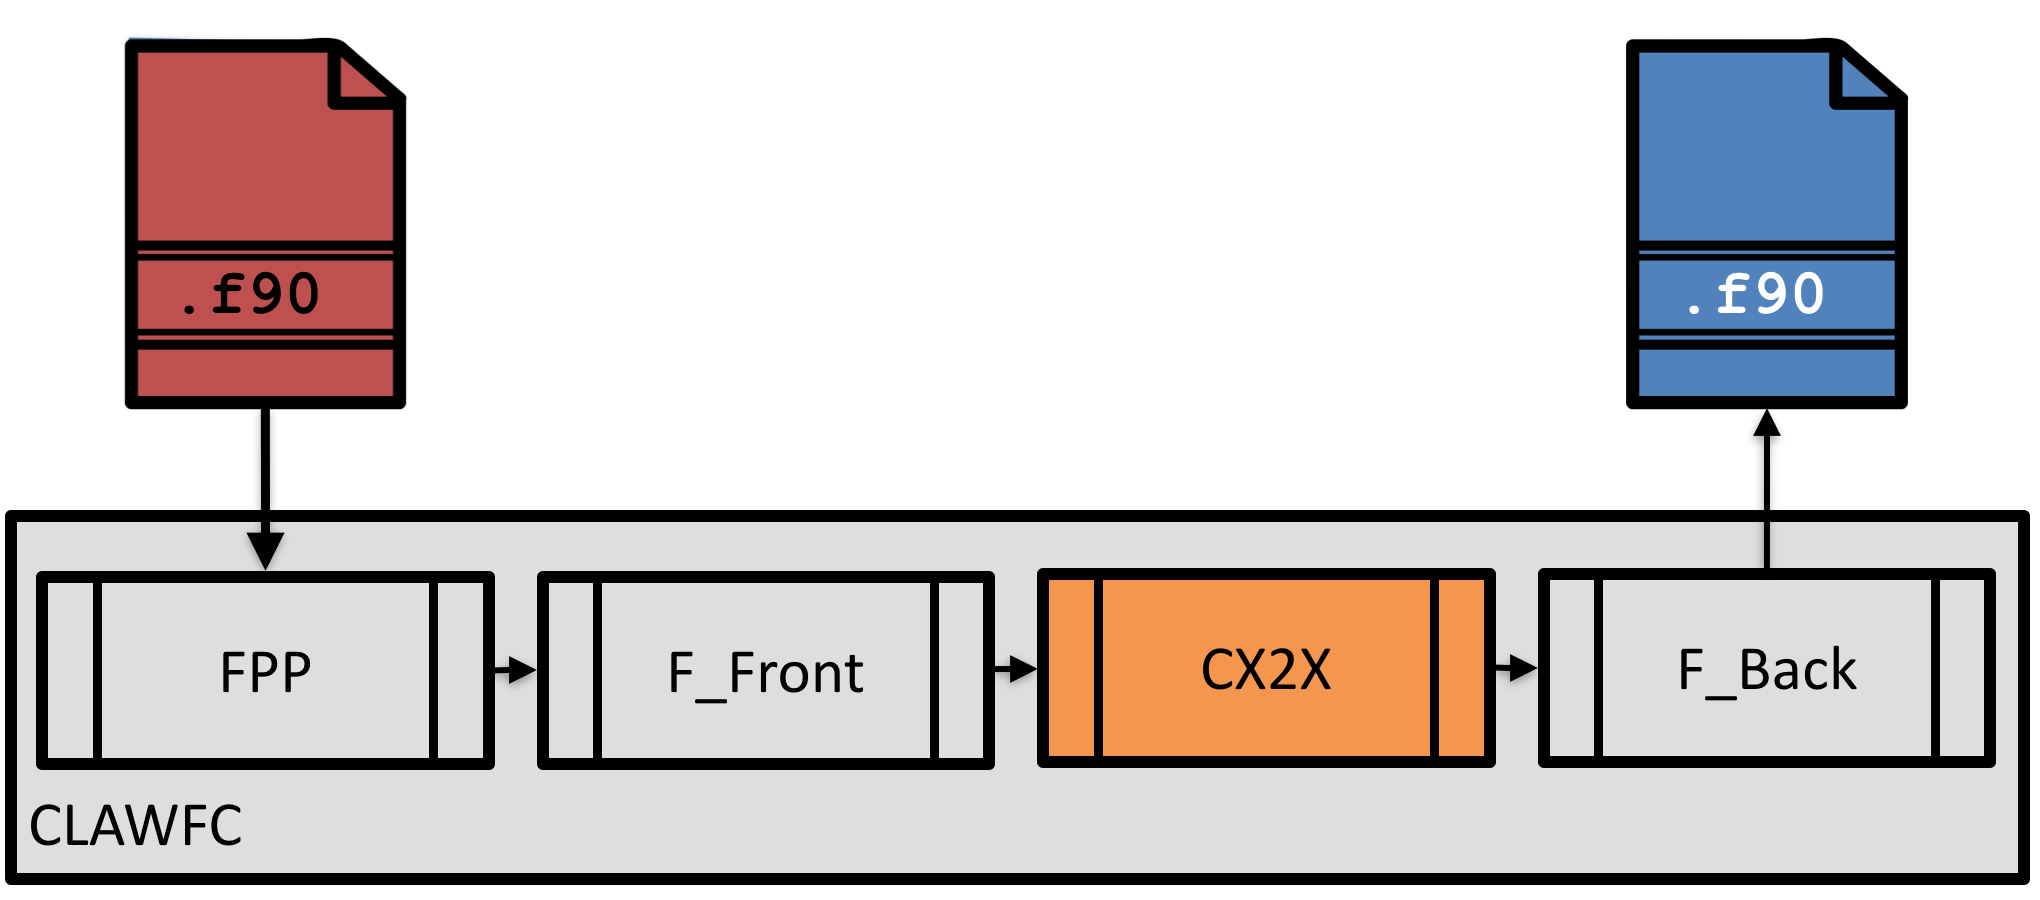
\includegraphics[width=0.8\textwidth]{resources/clawfc_global_workflow.png} \\
  \caption{CLAW FORTRAN Compiler main workflow.}
  \label{fig:clawfc_main_workflow}
\end{figure}

\section{CLAW \xcodeml to \xcodeml translator}
The \xcodeml to \xcodeml translator is the intelligence of the \clawfcomp. It understands the CLAW directive language and apply the corresponding transformation to the \xcodeml \gls{ast}.


\chapter{Transformation}
\section{Transformation application order}

\section{Add a transformation}
A transformation is always triggered by a directive. 

\chapter{\xcodeml and AST manipulation library}
As the \xcodeml \gls{ir} is based on the XML format, it can be manipulated with any language that can read and write XML files. It can even be manipulated by hand depending on the user's knowledge of the \xcodeml \gls{ir} specification. 
To ease this task, a small manipulation library is included in the \cx2x program. This library helps to traverse the \gls{ast}, add, modify or delete node.

\section{Traverse the \gls{ast}}

\section{Add nodes}

\section{Modify nodes}

\section{Delete nodes}

% GLOSSARY
\pagebreak
\glsaddall
\printglossaries

\emptypage
% FIGURES
\pagebreak
\listoffigures

%TABLES
\pagebreak
\listoftables

\emptypage
% LISTINGS
\pagebreak
\lstlistoflistings

% REFERENCES
%\input{references}

%\emptypage
%\input{appendix}

\end{document}
